%!TEX program = xelatex
%!TEX options = --shell-escape
\documentclass[10pt,aspectratio=169,mathserif]{beamer}		
\usepackage{nju}			                % nju template
\usepackage{ctex}                           % support Chinese
\usepackage{amsmath,amsfonts,amssymb,bm}    % math packages
\usepackage{color}			 				% support colored text
\usepackage{graphicx,hyperref,url}	
\usepackage[draft]{pdfcomment}              % would be helpful in presentation mode
% \usepackage[final]{pdfcomment}
\usepackage{caption}
\captionsetup[figure]{font=footnotesize}
\usepackage{amsmath}
\usepackage{multirow}
\newcommand{\xdownarrow}[2][]{%
\left.{#1}\right\downarrow{#2}}
\usepackage{url}
\usepackage{media9}
\usepackage{minted}                         % better source code highlighting


% If you have uncommon letter in name just like me...
\setCJKmainfont[ItalicFont=Adobe Kaiti Std, BoldFont=Adobe Heiti Std]{Adobe Song Std}
\setCJKsansfont{Adobe Heiti Std}
\setCJKmonofont{Adobe Fangsong Std}

\hypersetup{
  colorlinks,
  allcolors=.,
  urlcolor=blue,
  % linkcolor=green,
  % linkbordercolor=red,
  % pdfborderstyle={/S/U/W 1},
}


\newcommand{\pdfnote}[1]{\marginnote{\pdfcomment[icon=note]{#1}}}   % move the note away from the main content of your slide
\newcommand\blfootnote[1]{%
\begingroup
\renewcommand\thefootnote{}\footnote{#1}%
\addtocounter{footnote}{-1}%
\endgroup
}
% \newif\ifplacelogo % create a new conditional
% \placelogotrue % set it to true
\newcommand{\nologo}{\setbeamertemplate{logo}{}}    % command to set the logo to nothing


\beamertemplateballitem

% This would show a highlightened toc before each section
\AtBeginSection[]
{
  \begin{frame}
    \frametitle{目录}
    \tableofcontents[currentsection]
  \end{frame}
}


% Front page
\title[]{移动应用推广中流量劫持作弊行为的\\大规模检测与分析}
\subtitle{}
\author[]{赵旻睿}
\institute[COSEC]{南京大学网络合作与安全研究中心}
% \author{hakureicode@gmail.com}
\date{\today}
\logo{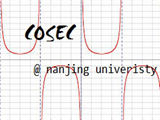
\includegraphics[height=1.5cm]{cosec.jpg}{\hspace{30pt}}}    % If you do not need logo, just comment out it

\begin{document}

\setbeamertemplate{headline}[nju theme no tos] 
\frame{\titlepage}

\nologo

\setbeamertemplate{headline}[nju theme]

\frame{\frametitle{目录}\tableofcontents}			

\section{Section 1}
\begin{frame}
  \frametitle{Section 1}

    In this slide, some important text will be
    \alert{highlighted} because it's important.
    Please, don't abuse it.

    \begin{block}{Remark}
      Sample text
    \end{block}

    \begin{alertblock}{Important theorem}
      Sample text in red box
    \end{alertblock}

    \begin{examples}
      Sample text in green box. The title of the block is ``Examples".
    \end{examples}

\end{frame}

\section{Section 2}
\begin{frame}[fragile]      % If you are using minted, remember to append fragile option to the frame
  \frametitle{Section 2}

    Houston, we have a problem.

    \vspace*{10pt}

    \begin{minted}[fontsize=\scriptsize]{java}
try {
    throw new Exception("blah");
} catch(Exception e) {
    for (StackTraceElement stackTraceElement: e.getStackTrace()) {
        // stackTraceElement.getClassName() stackTraceElement.getMethodName()
        // try to find Hook Frame in the calling stack
    }
}
    \end{minted}

    \blfootnote{\tiny \url{https://www.gutenberg.org/files/18269/18269-h/18269-h.htm\#p_347}}

\end{frame}

\section{Section 3}
\begin{frame}
  \frametitle{Section 3}
	   
    Example of pdfcomment
    \pdfcomment{
    blahblahblah, \textCR
    blahblah.}

\end{frame}

\subsection{Subsection 4}
\begin{frame}
  \frametitle{Subsection 4}

    Example of pdfnote
    \pdfnote{remember to say thankyou!!!}

\end{frame}

\setbeamertemplate{headline}[nju theme no tos] 
\begin{frame}
    \centering \large Thanks for watching!
\end{frame}

% If needed
\frame{\tableofcontents}

\end{document}
